\begin{savequote}[8cm]
I take lettuce, onions, tomato \\
Add a dab of mayo plus the fish fillet-o \\
Appetizing gray matter with a strange platter \\
The symmetry of energy with chemistry and plasma \\
 \qauthor{--- Edan, \textit{I see colours}} 
\end{savequote}

%Here we solved a one-dimensional Schr\"odinger equation for the nuclear degree of freedom along the phonon mode, and then combine the resulting thermalised probability density function (which includes zero point fluctuations and quantum tunnelling) with a band-gap deformation potential along this mode. 
%The method includes quantum nuclear motion, goes beyond the harmonic regime, but only contains the first-order contribution to the electron-phonon coupling of the band-gap deformation. 

\chapter{\label{ch:5-epcoupling}Electron-phonon and phonon-phonon coupling}
% see ziman electrons and phonons?
% https://journals.aps.org/rmp/pdf/10.1103/RevModPhys.89.015003

Excerpts of this chapter and Figures 2--4 are adapted from
\href{https://doi.org/10.1103/PhysRevB.94.220301}{Whalley, L. D., Skelton, J. M., Frost, J. M. and Walsh, A. (2016). Phonon anharmonicity, lifetimes, and thermal transport in \ce{CH3NH3PbI3} from many-body perturbation theory. \textit{Physical Review B}, 94(22).} © 2016 American Physical Society

Figures 1, 5--6 are adapted from
\href{https://doi.org/10.1021/acsenergylett.7b00862}{Frost, J. M., Whalley, L. D and Walsh, A. (2017). Slow Cooling of Hot Polarons in Halide Perovskite Solar Cells. \textit{ACS Energy Letters}, 2(12), pp.2647-2652.} © 2017 CC-BY

\section{Introduction} \label{ch5:introduction}

% simplest approximation is that there is no coupling. But then mobility too large. In reality scattering (see previous chapter)
%include v. brief overview of what each is and explain that it is linked to non-radiative recombination and other important processes, thermal transport.
In the simplest approximation of a semiconductor -- a single electron in a perfect lattice at zero kelvin -- electrons do not scatter and as a consequence they have infinite mobility. In the next best approximation, harmonic phonons are introduced. Now the electrons scatter from the phonons, and the electron mobility becomes finite. This electron-phonon interaction underpins many phenomena in condensed matter physics and materials science including carrier mobility, polaron formation, hot carrier thermalisation and carrier capture. However in the harmonic phonon approximation, the phonons do not interact with one another -- they have an infinite lifetime. To calculate thermal conductivity and understand how a polaron cools to equilibrium we need to consider anharmonic phonon-phonon interactions. Some processes involve both electron-phonon and phonon-phonon interactions; for example during non-radiative recombination, carrier capture and lattice relaxation proceed via the electron-phonon and phonon-phonon interactions. 

This chapter begins with an introduction to electron-phonon coupling, with coupling to the acoustic and optical phonon modes considered. This extends the MAPI-focused discussion in Section \ref{ch2epcoupling} to consider the broader underlying theory. Later in the chapter I show that there is strong coupling between the highly anharmonic phonon modes that are associated with octahedral tilting in MAPI and the electronic states at the band edge. 

Phonon-phonon coupling, and how this relates to hot-carrier cooling in MAPI, is also introduced. Using a simple classical model for heat diffusion, I show that the ultra-low thermal conductivity of perovskites can be used to explain the experimentally observed slow cooling of photoexcited above bandgap electrons.

% Can measure a temperature dependance in the electronic structure:, Peaks shift, Peaks broaden (shorter electron lifetime), There is a direct and indirect (through the change in volume) contribution to dE/DT. , For direct: See AHC theory., For the indirect what we are asking is the effect of thermal expansion. See monserrat work or Bi2Se3 where it is not negligible. For Si the expansion is negligible (Xavier Gonze)

\subsection{Electron-phonon coupling}
We have previously considered a system where the electronic and vibrational substates are decoupled. %the full wavefunction product of ht other two.
However to model electron-phonon interactions we must remove this approximation and employ a Hamiltonian that describres the coupled system. 
The crystal Hamiltonian can be split into three terms:\autocite{Cardona2010}
\begin{equation}
	\hat{H} = H_e+H_{ion}+H_{e-ion}.
\end{equation}
The electronic sub-system corresponds to non-interacting band electrons in a periodic lattice with energy $\epsilon_{n\textbf{k}}$. 
Using the formalism of second-quantisation this electronic Hamiltonian $H_e$ can be expressed in a relatively compact form:\autocite{Giustino2017}
\begin{equation}
H_e=\sum_{n\textbf{k}}\epsilon_{n\textbf{k}}\hat{c}^{\dagger}_{n\textbf{k}}\hat{c}_{n\textbf{k}}, 
\end{equation}
where $\hat{c}_{n\textbf{k}}\hat{c}^{\dagger}_{n\textbf{k}}$ is a number operator which tells us how many electrons are in a state with band index $n$ and crystal momentum $\textbf{k}$.
The lattice sub-system corresponds to non-interacting quantised harmonic vibrations (phonons) with energy $\hbar\nu_{\textbf{q}v}$ and can be expressed in the language of second quantisation as:
\begin{equation}
H_{ion} = \sum_{\textbf{q}v}\hbar\nu_{\textbf{q}v}(\hat{a}^{\dagger}_{\textbf{q}v}\hat{a}_{\textbf{q}v}+\frac{1}{2}),
\end{equation}
where $\hat{a}_{\textbf{q}v} \hat{a}^{\dagger}_{-\textbf{q}v}$ is a number operator which tells us how many phonons are in a state with branch index $v$ with crystal momentum $\mathbf{q}$.

To describe the interaction between the electron and phonon sub-systems it is assumed that the electrons respond instantaneously to the ionic motion.
This allows the electron-phonon interaction term of the Hamiltonian to be expressed as a Taylor series expansion of the electronic Hamiltonian:\autocite{Cardona2010}
\begin{equation}
H_{e-ion} = \sum_j\left(\frac{\partial H_e}{\partial R_j}\right)\bigg\rvert_{R_{j0}}\cdot\delta R_j\ldots
\end{equation}
where $\delta R_j$ is the displacement of ion $j$ from the equilibrium position $R_{j0}$.
The zeroth order term is not included as this is the interaction of the electrons with the static lattice and is already included in the electronic Hamiltonian.
The first order term of the expansion describes the lowest-order process that involves coupling between the electron and phonon sub-system, and corresponds to the scattering of a single electron by a simultaneous creation or annihilation of a single phonon.
In second quantised form electron-phonon coupling term can be expressed as:\autocite{Giustino2017}
\begin{equation} \label{HamiltonianEP}
H_{e-ion} = N_p^{-\frac{1}{2}}\sum_{\substack{\textbf{k},\textbf{q} \\ m,n,v}}g_{mnv}(\textbf{k},\textbf{q})\hat{c}^{\dagger}_{m\textbf{k}+\textbf{q}}\hat{c}_{n\textbf{k}}(\hat{a}_{\textbf{q}v}+\hat{a}^{\dagger}_{-\textbf{q}v}).
\end{equation}
The matrix element $g_{mnv}(\textbf{k},\textbf{q})$ determines the strength of the coupling and $N_p$ is the number of unit cells in the supercell. $\hat{a}_{\textbf{q}v}$ and $\hat{a}^{\dagger}_{-\textbf{q}v}$ are the operators that destroy and create phonons, whilst
$\hat{c}_{n\textbf{k}}$ and $\hat{c}^{\dagger}_{m\textbf{k}+\textbf{q}}$ are the operators that destroy and create electrons.

Unfortunately Equation \ref{HamiltonianEP} does not tell us how to calculate the electron-phonon matrix $g_{mnv}(\textbf{k},\textbf{q})$. The first expression for the matrix elements was derived by Bl\"{o}ch in 1929:\autocite{Giustino2017}
\begin{equation}
g_{mnv}(\textbf{q}) = -i\left(\frac{\hbar}{2N_pM_\kappa\nu_{\textbf{q}v}}\right)^{\frac{1}{2}}\textbf{q}\cdot\textbf{e}_{\kappa v}(\textbf{q})V_0,
\end{equation}
where $V_0$ is an average effective potential experienced by the electrons in the crystal, $M_\kappa$ is the mass of the $\kappa$th nucleus and $\textbf{e}_{\kappa v}(\textbf{q})$ is a phonon eigenvector. The expression is derived for a monovalent metal with one atom in the unit cell and where the Kohn-Sham wavefunctions can be approximated by free electrons,\autocite{Giustino2017,Wallace1963} and as a result of this the expression is independent of the electron momentum.%p.92

The electron-phonon coupling term in Equation \ref{HamiltonianEP} contains a summation over all states in the electronic and vibrational Brillouin Zones. Considering all possible states is computationally intractable for many systems of interest, but the problem can be simplified by only considering the terms which make the most dominant contributions. In the case of covalent materials, it is assumed that the dominant interaction is between long wavelength acoustic phonon modes and electronic states. For ionic materials it is assumed that the dominant interaction is with the electric field generated by longitudinal optic phonons.

\subsubsection{Acoustic deformation potential scattering}  
 In 1950 Bardeen and Shockley introduced the `deformation potential' method,\autocite{Bardeen1950} which gives an approximation to $V_0$ for semiconductors where the dominant electron-phonon scattering mechanisms involve long wavelength acoustic phonons.\autocite{Giustino2017} In this approach average effective potential for a unit cell of volume $\Omega$ is given by:
\begin{equation} \label{couplingterm} 
   V_0 = \Omega\frac{\partial\epsilon_{n\textbf{k}}}{\partial\Omega}.
\end{equation}

The deformation potential in Equation \ref{couplingterm} can be determined empirically or calculated from first principles. 
%The coupling term $g$ is given by 
%\begin{equation}
%    q_{mnv}(k,q) = \langleu_{mK=q}|\Delta_{qv}v^{KS}|u_{nk}\rangle_{uc}
%\end{equation}

\subsubsection{Fr\"{o}lich interactions}  
In the Fr\"{o}lich polaron model a free electron interacts with the electric field generated by dispersionless longitudinal optic (LO) phonons.
This interaction only occurs in ionic crystals, where atomic displacements generate long-range electric fields.
In this model the effective potential is replaced with
\begin{equation}
    V_0 = \left[\frac{e^2M_k\nu^2_{\textbf{q}v}}{\epsilon_0\Omega}\left(\frac{1}{\epsilon^{\infty}}-\frac{1}{\epsilon^0}\right)\right]^{\frac{1}{2}}\frac{1}{|\textbf{q}|^2}
\end{equation}
where $\epsilon_0$,$\epsilon^0$ and $\epsilon^{\infty}$ are the vacuum, static, and high-frequency permittivities respectively.

MAPI is a soft material, with structural distortions and dynamic disorder at room temperature, so electron-phonon interactions are expected to be significant.
Furthermore, long charge carrier diffusion lengths (up to \SI{10}{\micro\metre}) but modest mobilities (up to \SI{100}{\square\cm\per\volt\per\second}) point to strong electron-phonon interactions.\autocite{Brenner2015} 
Photoluminescence studies of formamidinium-lead-iodide suggest that acoustic deformation potential scattering makes only a minor contribution to electron-phonon interactions at room temperature,\autocite{Wright2016}
as there is decreased electron-phonon coupling at temperatures below the relevant LO phonon for Fr\"{o}lich coupling. This suggests that Fr\"{o}lich interactions dominate, and is supported by a theoretical calculation which predicts a LO-phonon limited mobility in line with experiment.\autocite{Frost2017b}
%A recently developed formalism to study polarons using coupling terms calculated from density functional perturbation theory has confirmed the validity of the Frolich Hamiltonian for large polarons. (giustino)

% Robert Lobronvnic Optical phonon modes hbarw are occupied at kT @ room temperature: RARE
\subsection{Hot carrier cooling in hybrid halide perovskites}

Halide perovskites display unusual cooling kinetics for electrons photo-excited above the bandgap.
The cooling of these `hot' electrons is slower than that observed in other semiconductors and this has been attributed to a `hot phonon bottleneck'.\autocite{Yang2016e,Yang2017a} % 
As a result of strong Fr\"{o}lich coupling between the electronic and optical phonon modes, hot carrier cooling in the hybrid perovskites does not occur through a single process but can be split into three stages: i) transfer of energy from the electron to optical phonons (via the electron-phonon Fr\"{o}lich interaction); ii) optical phonon decay into acoustic phonons (phonon-phonon interaction); iii) acoustic phonon propagation (phonon-phonon interaction).

The hot phonon bottleneck results from the equilibriation of hot carriers with a non-equilibrium phonon population;
Fr\"{o}lich interactions strongly couple the hot electrons to longitudinal optical (LO) phonons, but the LO phonons are not able to dissipate their heat. 
Poor thermal transport could be attributed to weak coupling between the optical and acoustic phonon modes, or to reduced acoustic phonon mode propagation so that the phonon modes are able to re-heat carriers.
In either case, we would expect two timescales to appear experimentally; fast initial thermalisation with optical phonons via the Fr\"{o}lich interaction, followed by slower cooling to equilibrium with the extended bulk solid (Figure \ref{cooling_schematic}). Here we make a distinction between thermalisation, which we define as equilibration with local phonon modes, and cooling, which is equilibration with the extended bulk solid.

\begin{figure}[h!]
\centering
  \includegraphics[width=0.7\columnwidth]{figures/ch5/f1.pdf}
  \caption[Schematic of the hot carrier cooling model]{Physical processes involved with the photogeneration of charge carriers in hybrid halide perovskites: i) exciton generation; ii) exciton dissociation, hot polaron formation and thermalisation; iii) hot phonon cooling to the band edge. Note that we make a distinction between thermalisation, which we define as equilibration with local phonon modes, and cooling, which is equilibration with the extended bulk solid. Together, they form the hot carrier relaxation process. Figure prepared by Aron Walsh.}
\label{cooling_schematic}
\end{figure}

%    Cooling is ten times slower in FAPI than in Caesium-based. Postulate that up-conversion of low-energy phonons is responsible, and this is possible dues to overlapping phonon branches of organic cations. Also due to blocking of phonon propagation with ultralow thermal conductivity. Two stages in cooling are identified; the first is independant of fluence whlst the second is not. First is attributed to Fr\"{o}lich phonon emission (electron and LO phonon coupling). Similar between Cs and organic as the electronic band structure near the band edge is dominated by the inorganic PbI framework. Second stage appears when sufficient fluence is used. Higher fluence means longer cooling lifetime.
 %   MAPI has a poor hot carrier response cmopared to FAPI. .MAPI is found to have much faster cooling time than FAPI. This is explained by lattice defects. Faster carrier relaxation indicates a large number of above bandgap defects which provide relaxation pathways for hot carriers. A second power dependant hot phonon bottleneck effect is found.
% Carrier thermalisation --> LO emission ---> acoustic phonon decay ---> local lattice heating ---> acoustic phonon propagation and the heat is dispersed. So three stages: (1) carrier-phonon (Fr\"{o}lich interaction) (2) Optical phonon decay to acoustic phonons (3) acoustic phonon propagation.
 % Things that can increase the overall cooling period are (1) thermal isolation between optical phonon and carriers (achieved through large polaron effect). Ruled out here as power independant second stage but not first. (2) reducing the phonon dos (opening the phonon bandgap using large atomic mass differences, gap twice the highest acoustic phonon). Not seen here. (3) acoustic up-conversion to optical phonons (local lattice heat doesn't dissipate to surroundings but reheats carriers)
   % Optical phonon modes in hybrids show a relatively flat band compared with inorganic case - non-propagating vibrations on the organic cation. Cascade decay of LO phonons may slow cooling.
 %   Hybrid phonon modes which are covibrations between organic and inorganic lattice. Excited by phonon-phonon scattering events. Show littel dispersion and have good overlap with coustic branches. So acoustic phonons scatter to optical states. Anharmonic phonon-phonon scattering, low thermal conductivity, means that propagation blocked and increase probabilty of up-transition.


%\begin{figure}[h!]
%\centering
%  \includegraphics[width=0.7\columnwidth]{C05/figs/f1.pdf}
%  \caption{Reproduced from reference \cite{Whalley2017a}.}
%  \label{cooling_schematic}
%\end{figure}
%\section{Summary}

% what is happening in this chapter: calculated for MAPI.
% Modes are the soft modes: Anharmonic soft tilting modes are characteristic of the perovskite material family. For cubic perovskite with a unit cell of The tilting corresponds to opposite tilting in neighbour cell, so happens at M (0.5,0,0) amd R (0.5,0.5,0). Hybrid halide perovskites have double-well potentials associated with octahedral tilting of the inorganic lattice. These are located at the $M$ and $R$ point in the brillouin zone.
%We use a `mode mapping' approach to distort the structure along the $M$ and $R$ eigenvectors and track the change in bandgap as a function of the normal mode coordinate $Q$ (which corresponds to the amplitude of the phonon mode).


\section{Methods}

\subsection{Lattice dynamics calculations}

Harmonic lattice-dynamics calculations were performed with the \textsc{Phonopy} package.\autocite{Togo2015} Displacement steps of \SI{0.01}{\angstrom} were used to evaluate the second-order force-constant matrix using the finite-displacement method. This step size is commonly reported in the literature\autocite{Togo2015,Skelton2017} and is the default value in the \textsc{Phonopy} package.
A $4\! \times\! 4\! \times\! 4$ supercell expansion was used to compute the second-order force constants (72 displacements in a 768-atom cell).
Forces were computed within the Kohn-Sham density-functional theory (DFT) formalism as implemented in the \textsc{VASP} code,\autocite{Kresse1996a} using the scalar relativistic corrections given in Section \ref{bgdefmethod}.
The valence wavefunctions were expanded in a plane-wave basis set with a 800 eV cut-off and the exchange and correlation interactions between electrons were modelled using the PBEsol exchange-correlation functional.\autocite{Perdew2008a}
The electronic Brillouin zone was evaluated at the $\Gamma$-point, and a total-energy convergence criterion of $10^{-8}$ eV was used.

\subsection{Calculation procedure for the bandgap deformation potential} \label{bgdefmethod}

Density-functional perturbation theory (DFPT) is a method commonly used to calculate the electron-phonon coupling. However DFPT assumes a small harmonic response for the perturbative treatment to be correct and for anharmonic phonon modes this assumption does not hold.
For MAPI, where the range of motion is large and anharmonic, the `frozen phonon' method can be used: here the energy of the valence and conduction bands are tracked as the crystal lattice is distorted along a single phonon mode to give a bandgap deformation potential.

\textsc{Phonopy}\autocite{Togo2015} was used to calculate the harmonic phonon eigenvalues and eigenvectors, as outlined above. ModeMap scripts available online\autocite{ModeMap} were used to generate a sequence of structures along the phonon eigenvectors at the $M$ and $R$ points in reciprocal space. 

The deformation potentials were calculated by following the phonon mode vectors and mapping the change in bandgap as a function of normal mode coordinate $Q$.
Bandgaps were computed within the Kohn-Sham density-functional theory (DFT) formalism as implemented in the \textsc{VASP} code.\autocite{Kresse1996a}
The valence wavefunctions were expanded in a plane-wave basis set with a 700 eV cut-off and the exchange and correlation interactions between electrons were modelled using the PBEsol exchange-correlation functional\autocite{Perdew2008a} ($Q$ from 0 to 150 amu$^{\frac{1}{2}}$ \AA) and a screened hybrid functional (HSE06)\autocite{Heyd2004a,Heyd2005a} ($Q$ from 0 to 69 amu$^{\frac{1}{2}}$ \AA).
Scalar-relativistic corrections were used for the core electrons within the projector augmented-wave (PAW) formalism,\autocite{Blochl1994} with the outermost s and p electrons of C, N and I, and the outermost s, p and d electrons of Pb, being treated as valence. 
The PAW projection was applied in reciprocal space (\textsc{LREAL = .FALSE.} in \textsc{VASP}).
Spin-orbit coupling, which strongly affects the unoccupied conduction band, was considered for the PBEsol functional.
A Monkhorst-Pack \textit{k}-point grid, with a $\Gamma$-centered $6 \times 6 \times 6$ grid, was used to integrate the electronic Brillouin zone.
A total-energy convergence criterion of $10^{-8}$ eV during the electronic minimisation was found to be necessary to remove noise in the absolute electronic eigenvalues.
A least-squares polynomial fit using the \textsc{Python} library \textsc{Numpy} was applied to the symmetrised data.

The Cartesian displacement of atoms in a $N_a$ atom unit cell for a phonon mode with amplitude $Q$ scales as $\frac{Q}{\sqrt{N_a}}$. %link to phonopy documentation here
However, as evidenced and discussed further in Appendix \ref{app:6-SCcompare}, the average bandgap for a given temperature does not scale with supercell size.

\subsection{Classical model for hot carrier cooling}
The hot carrier cooling rate was modelled classically. The polaron was considered as a hot-sphere in a continuum of ambient-temperature material. This reduces the problem to one-dimension, where the exponent is weighted by the $r^2$ increasing shell of available states over the surface of the sphere. 
The initial “top hat” heat distribution was convolved with a Gaussian kernel to give an analytical expression for the evolution of hot carrier energy with time. The analytical expression and derivation is given in Appendix (\ref{app:2-diffusion}).
The rate of cooling was determined by the diffusivity $D$:
\begin{equation}
    D = \frac{\kappa}{\rho c_p}
\end{equation}
where $\kappa$ is the thermal conductivity, $\rho$ is the material density, and $C_p$ is the specific heat capacity.

\section{Results}
\subsection{Anharmonic bandgap deformation potential} \label{ch5bdp}
Deformations along the soft acoustic phonon modes at $q$-points $M$ and $R$ in reciprocal space are considered, which correspond to in-phase and out-of-phase tilting of the inorganic octahedra respectively (Figure \ref{ch5phonondisp}).
The potential energy is plotted as a function of $Q$, which describes the amplitude of the displacement along a given phonon mode.\autocite{Whalley2016}
To reduce the computational cost we take advantage of the symmetry of the double well potential energy surface (Figure \ref{fig2}) and consider distortions along positive $Q$ values only. The corresponding single-well potential energy surface can be found in Appendix \ref{app:6-SCcompare}.

\begin{figure}[h]
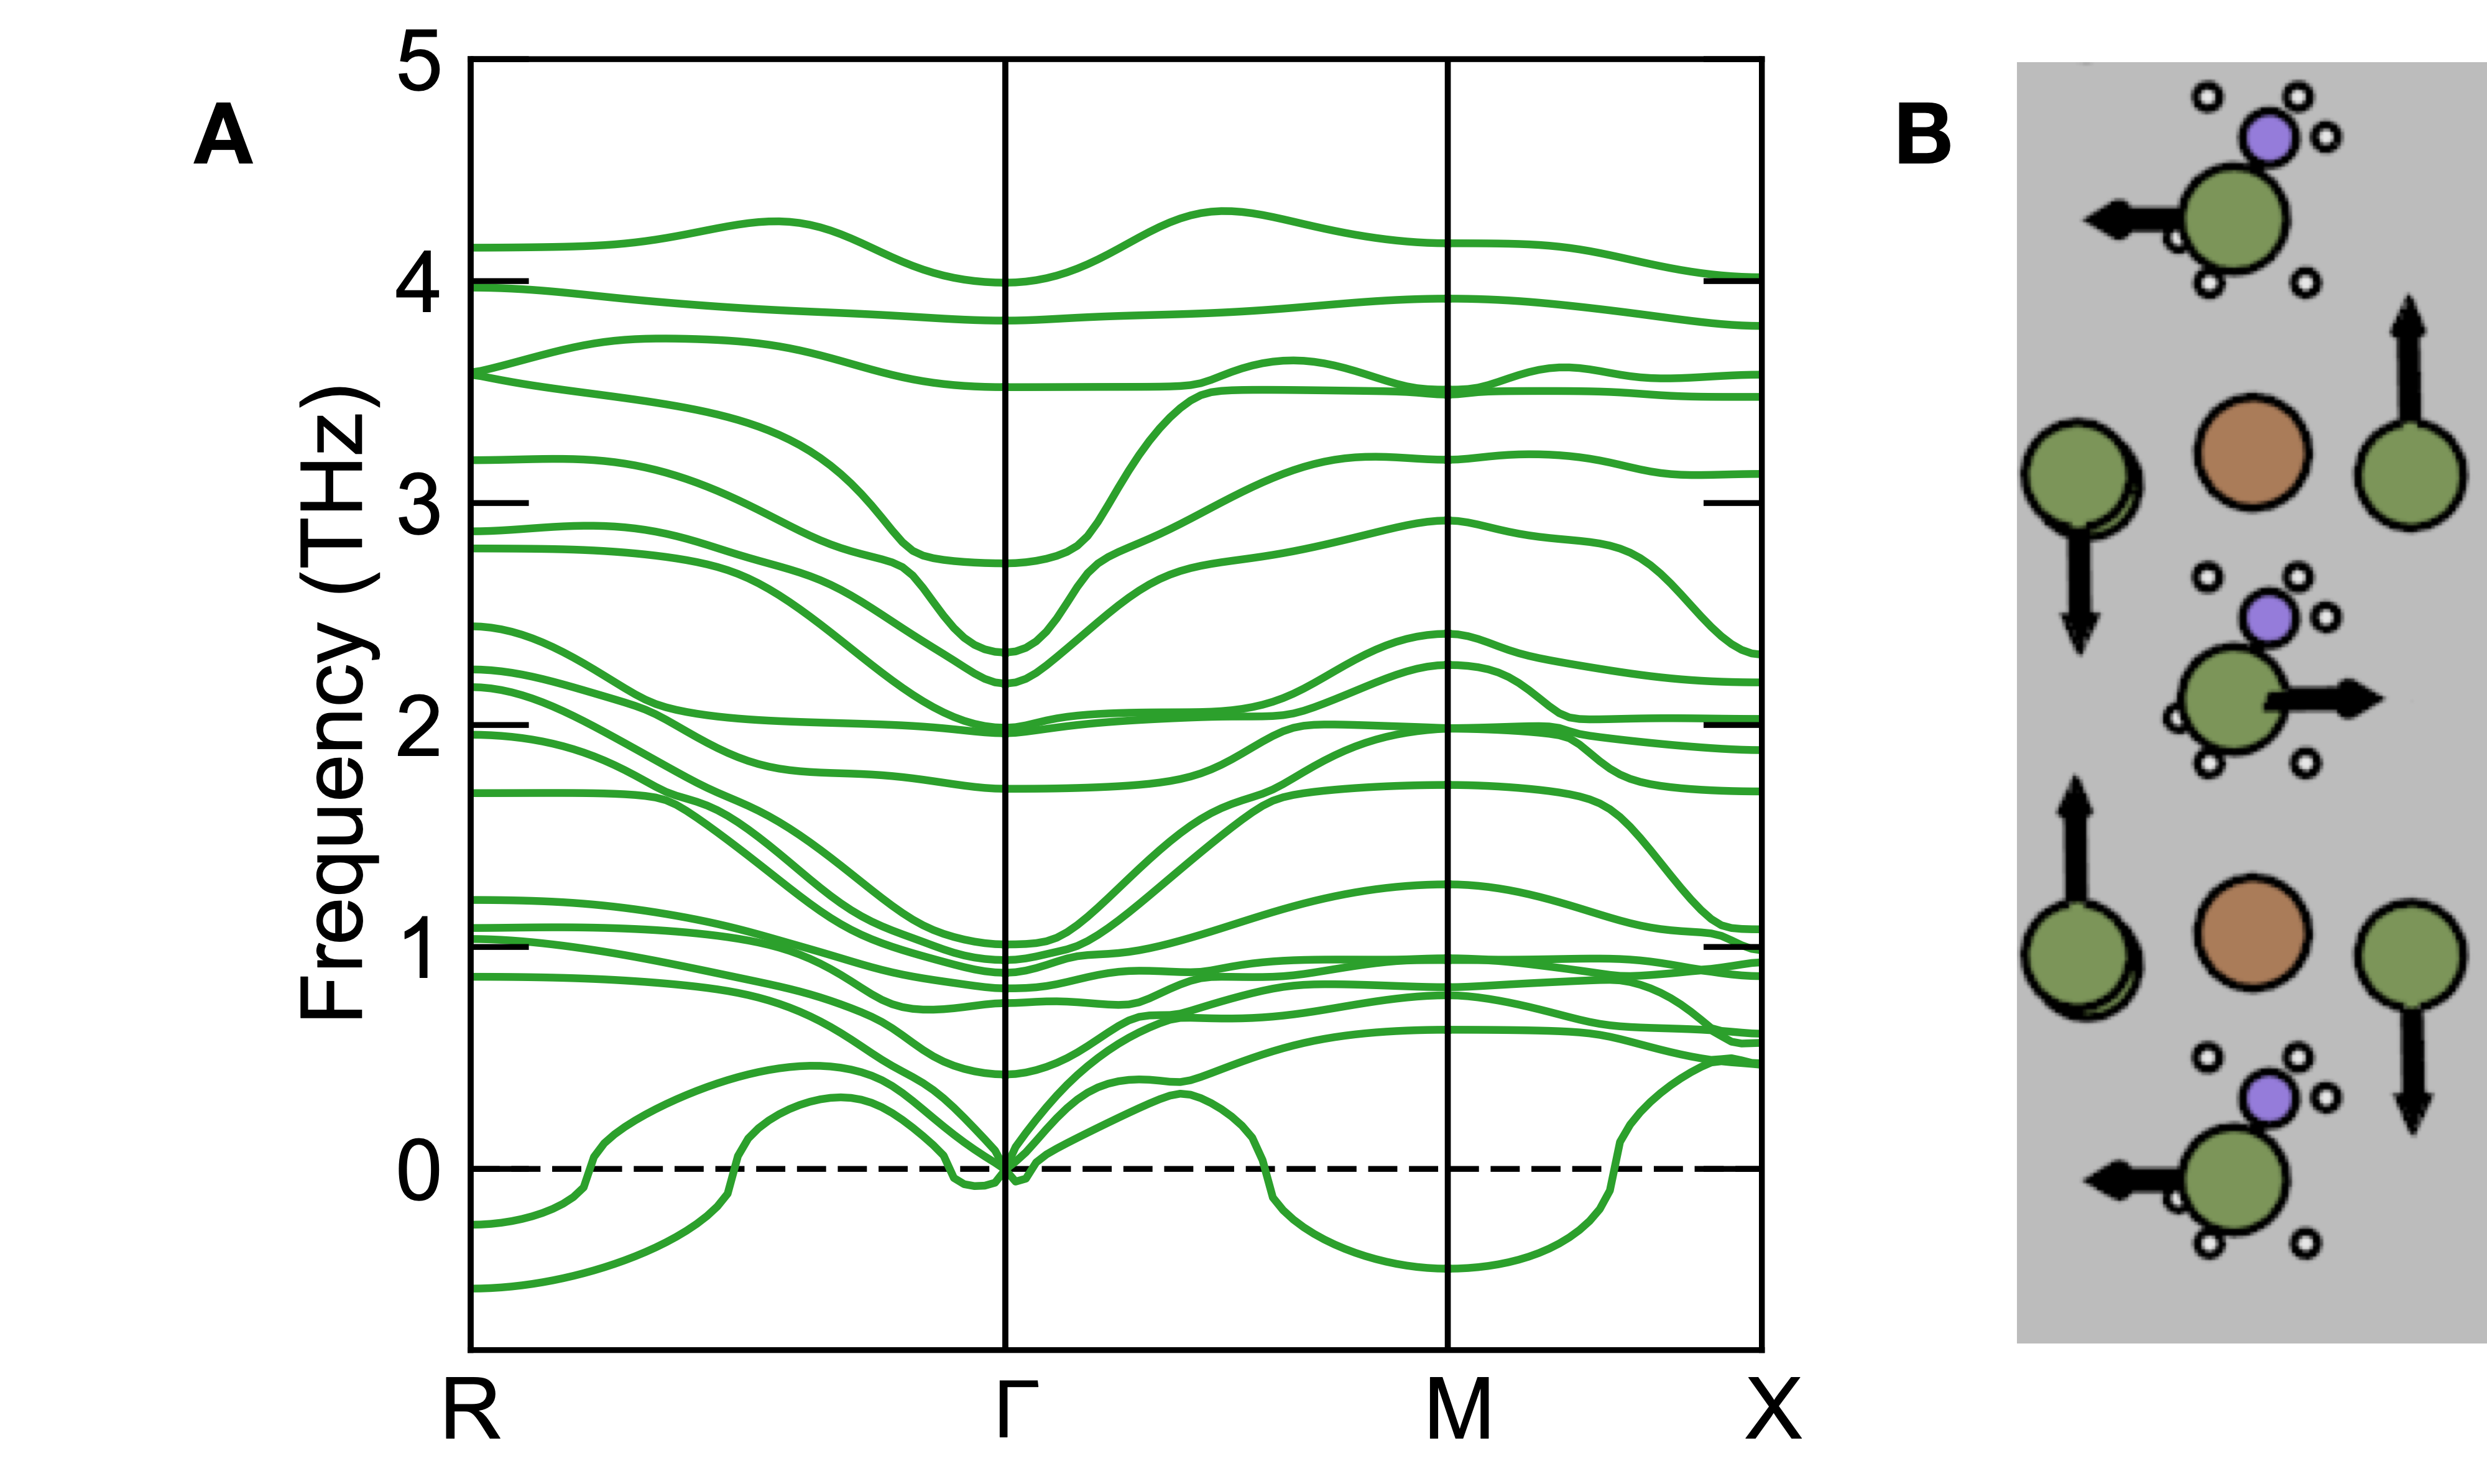
\includegraphics[width=0.8\textwidth]{figures/ch5/phonon_band.png}
\caption[Harmonic phonon dispersion and eigenvectors at the $M$ and $R$ $q$-points]{\label{ch5phonondisp} A) Harmonic phonon dispersion for MAPI. The bandgap deformation potentials are calculated for distortions along the imaginary mode eigenvectors at $q$-points $M$ and $R$ in reciprocal space. In the Fr\"{o}lich polaron model for MAPI phonon frequencies up to 5THz are considered, as wavenumbers above this correspond to the molecular vibrations of the organic cation.\autocite{Leguy2016} The imaginary modes at the $\Gamma$-point are a result of numerical noise. This image was generated using the \textsc{sumo} software package.\autocite{sumo2018} B) Eigenvector for the imaginary phonon mode at the $M$ point in the Brillouin zone. The green and brown atoms correspond to iodine and lead, respectively. The remaining atoms form the inorganic cation. The magnitude of the vector arrow is increased by a factor of three for clarity, and only the motion of the inorganic cage is considered. This image was generated using the \textsc{ascii phonons} package available at \url{https://github.com/ajjackson/ascii-phonons}.

}
\end{figure}

The change in bandgap as a function of normal mode coordinate $Q$ is plotted in Figure \ref{ch5figs1}. 
We find that the bandgap $E_\mathrm{g}(Q)$ is well described as quadratic over small $Q$, but that a bi-quadratic term is required to reproduce the correct behaviour at large $Q$ (Table \ref{RSS}). 
The significance of the bi-quadratic term is apparent when calculating the average bandgap as a function of temperature (Section \ref{ch5coupling}), as the quadratic fit leads to a predicted room temperature bandgap shift twice as large as that for the bi-quadratic fit.
% why does it broaden?

The total bandgap deformation is split into separate contributions from the conduction and valence bands (i.e. electron and hole coupling) in Figure \ref{ch5figs1}.
The electrostatic summation under periodic boundary conditions 
does not allow for the determination of absolute electron eigenvalues, and so a reference energy is needed to track the change in eigenvalue across calculations.  
We track the change in the valence- 
and conduction-band energies with respect to the Pb 3d deep-lying core states.
Fitting a quadratic function to the band energies shows the electron-phonon coupling 
to be roughly three times that of the hole-phonon coupling (i.e. the change in the conduction-band energy is three times the change in valence-band energy). %could do pdos here - why is coupling larger to the CB?? covalent interaction of p-states??

A similar bandgap deformation is found for the \textit{M} and \textit{R} modes (Table \ref{RSS}). This indicates that the out-of-phase tilting for successive planes in the \textit{R} mode has little additional effect on the gap and that the local tilting dominates the interaction.

\begin{figure}[h]
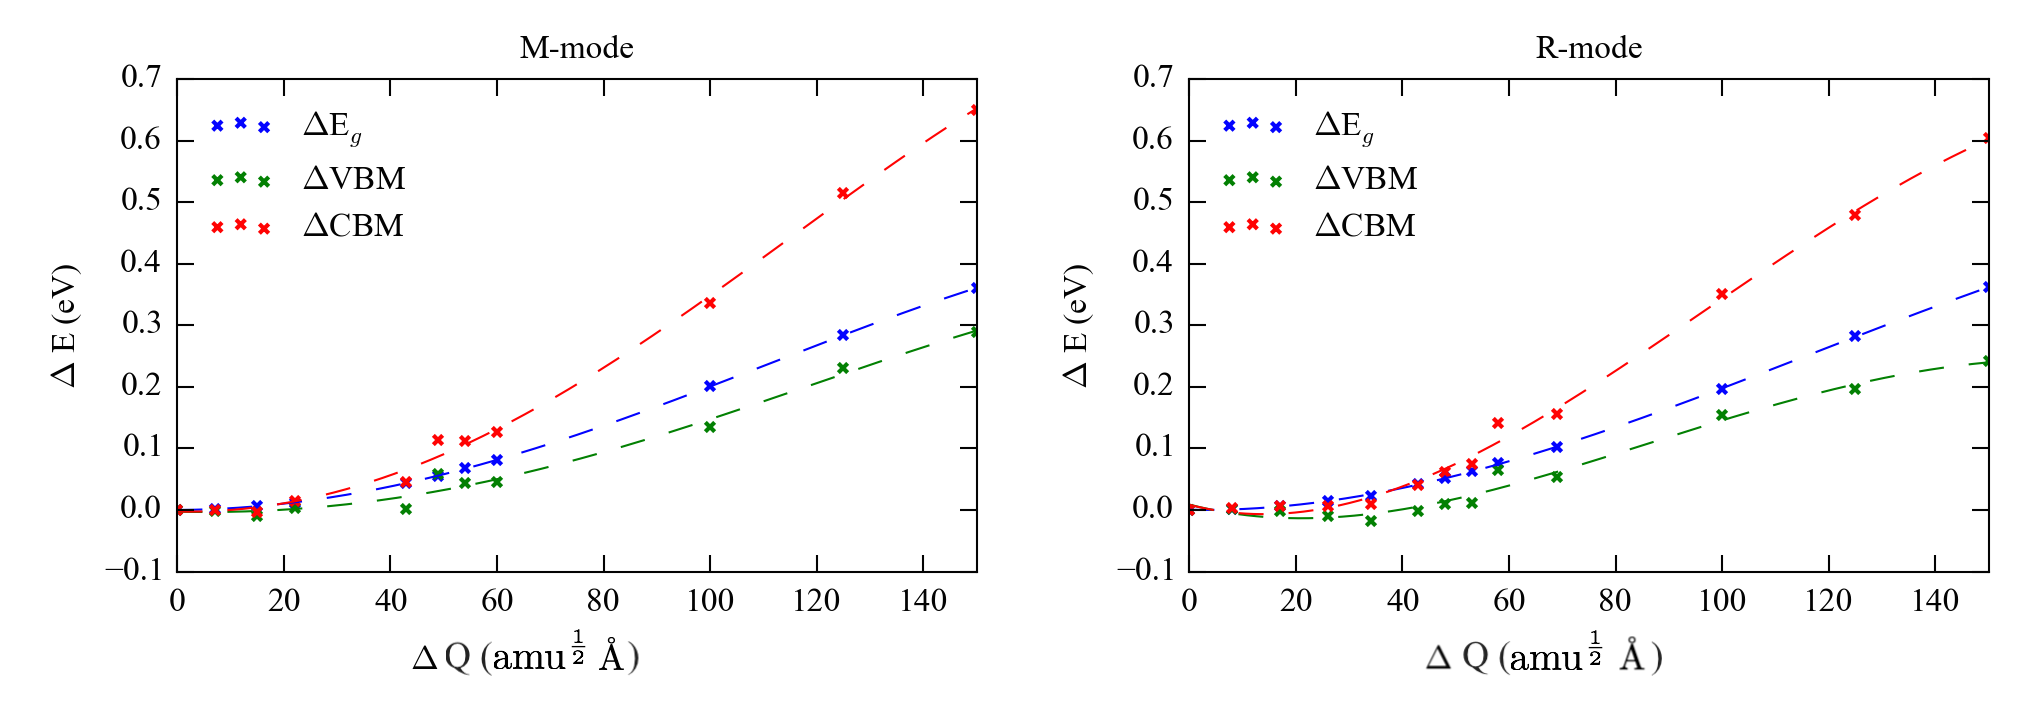
\includegraphics[width=\textwidth]{figures/ch5/fig_s3.png}
\caption[Bandgap deformation potential]{\label{ch5figs1}
Energy change ($\Delta$E) as a function of the normal-mode coordinate $Q$ of the valence-band maximum ($\Delta$VBM), conduction-band minimum ($\Delta$CBM), and bandgap ($\Delta$E$_g$) obtained from calculations using the PBEsol functional.
The energies of the band extrema have been referenced to the energy of the Pb 3d core states.
}
\end{figure}

\begin{table}[ht] \centering
 \caption[Residual sum of squares for quadratic and bi-quadratic fits to the bandgap] {Residual sums of squares (RSS) for quadratic and biquadratic fits to the data in Figure \ref{ch5figs1}. A smaller RSS indicates a better fit of the model to the data.}
  \label{RSS} 
 \begin{tabular}{cccc} 
 \toprule
 
  \multicolumn{1}{c}{} & $\Delta$VBM & $\Delta$CBM & $\Delta$E$_g$ \\
  \midrule
 \multicolumn{1}{c}{} & \multicolumn{3}{c}{$M$} \\

 Quadratic & $4.1 \times 10^{-3}$ & $ 1.1 \times 10^{-2}$ & $3.7 \times 10^{-3}$ \\

 Biquadratic & $3.2 \times 10^{-3}$ & $2.9 \times 10^{-3}$ & $2.0 \times 10^{-5}$ \\

 \midrule
 
  \multicolumn{1}{c}{} & \multicolumn{3}{c}{$R$} \\

 Quadratic &   $9.8 \times 10^{-3}$& $2.0 \times 10^{-2}$& $3.5 \times 10^{-3}$\\

 Biquadratic & $6.4 \times 10^{-3}$ &$6.0 \times 10^{-3}$ & $6.0 \times 10^{-5}$\\
 
 \bottomrule
 \end{tabular}
 \end{table}

For most semiconductor materials the bandgap decreases with temperature. This is attributed to bonding at the frontier orbitals, with the CBM composed of bonding states and VBM composed of antibonding states, so that thermal expansion leads to a decrease in VBM energy and increase in CBM energy.\autocite{Francisco2019}
In contrast, relativistic calculations for MAPI predict an `inverted' bandstructure with a VBM composed of antibonding hybridised Pb 6$s$- and I 5$p$ orbitals and a CBM dominated by the non-bonding 6$p$-orbitals of lead (Figure \ref{ch5pdos}).\autocite{Brivio2013}
As we distort the pseudo-cubic structure along the $M$ or $R$ phonon modes, the Pb-I bond length increases (Table \ref{ch5bondlength}), which indicates that there should be a decrease in CBM and VBM energies, contrary to the predicted energy increases.

Band edge energies as a function of various normal mode distortions have been investigated for the metal halide perovskite \ce{CsPbI3}, which shares the same VBM and CBM orbital character as MAPI.\autocite{McKechnie2018} For displacements along the normal phonon mode corresponding to octahedral twisting (iodine motion) around Pb, there is: i) a significant increase in the CBM energy; ii) a decrease Pb $p$-orbital character at the CBM; iii) an increase in I $p$-orbital character at the CBM. The increase in CBM energy is attributed to a reduction in Pb-$p$ character, as a result of reduced spin-orbit coupling. However tests on MAPI for two different descriptions of electron exchange and correlation and one including spin-orbit coupling, shows similar behaviour with respect to band deformation (Table \ref{ch5allxc} and Figure \ref{Egtheory}). 
Instead, we attribute the increase in energy to a decrease in orbital overlap between the Pb 6$p$-states, leading to a less dispersive band and decreased band width.
The increase in the VBM site energy could be attributed to the hybridised Pb 6$p$- and I5$p$ bonding orbitals which lie lower in the valence band,\autocite{Wang2015i} although further calculations to predict the orbital character as a function of phonon mode displacement are needed to confirm this hypothesis.
%useful lit: https://pubs.acs.org/doi/full/10.1021/acs.chemmater.6b00968 / https://journals.aps.org/prb/abstract/10.1103/PhysRevB.88.165203
%could look at Pb-Pb bond length also

\begin{figure}[h] \centering
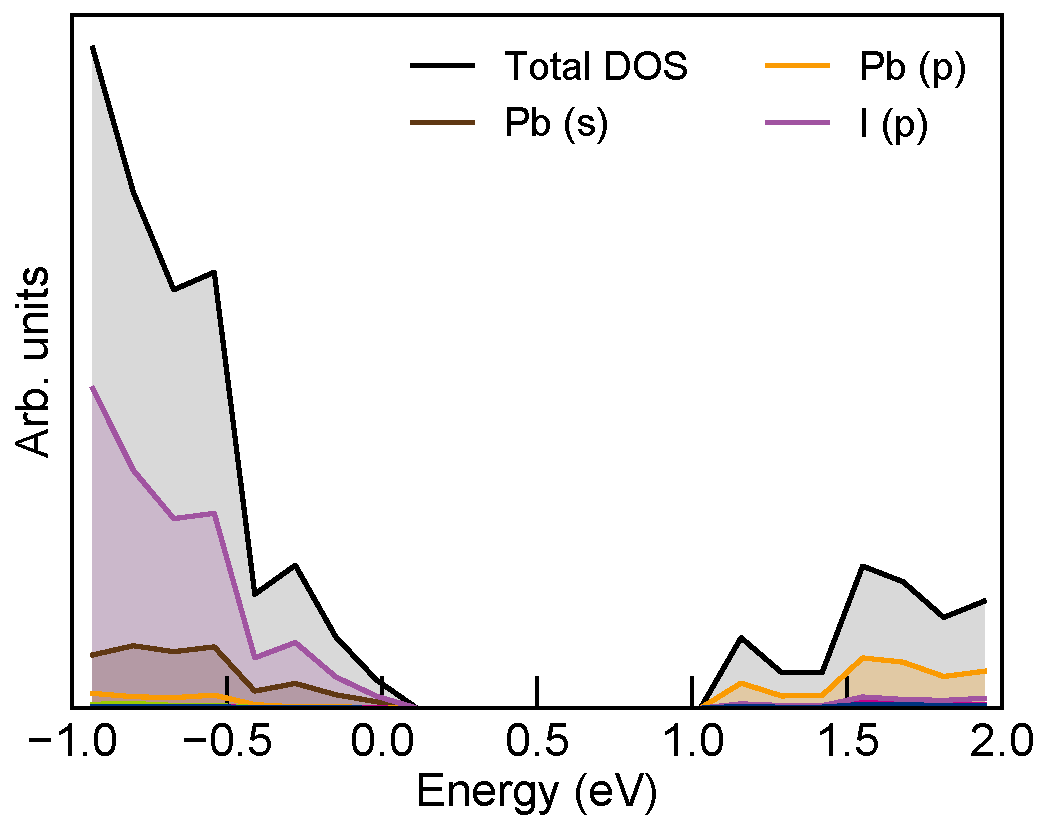
\includegraphics[width=0.6\textwidth]{figures/ch5/dos.pdf}
\caption[Total and projected density of states]{\label{ch5pdos}
Total density of states for \ce{CH3NH3PbI3}, including projections onto I $p$-orbitals and Pb $p$- and $s$-orbitals. Calculation uses the HSE06 exchange-correlation functional and includes spin-orbit coupling. Calculation parameters are those used for the bandstructure calculation in Section \ref{ch4:methods}.
}
\end{figure}

\begin{table}[h]  \centering
\caption[Pb-I bond lengths] {Pb-I bond lengths in MAPI for the pseudo-cubic and distorted structure. Distortion is along the M-mode with an amplitude of $64\ \textrm{amu}^{\frac{1}{2}}\AA$. Two bond lengths are not adjusted as the Pb-I1 and Pb-I4 bonds form an axis of rotation. }
\label{ch5bondlength}
\begin{tabular}{lcccccc} 
    \toprule
    &   \multicolumn{6}{c}{Bond} \\
 & Pb1-I1 & Pb1-I2 & Pb1-I3 & Pb1-I4 & Pb1-I5 & Pb1-I6 \\ 
    \midrule
Pseudo-cubic bond length ($\AA$) & 3.215 & 3.077 & 3.140 & 3.174& 3.25&3.141 \\
Distorted bond length ($\AA$)& 3.215& 3.107&3.185 & 3.174 & 3.283&3.143 \\
Difference ($\AA$) & 0 &+0.03 &+0.045 &0 &+0.033 &+0.002 \\
    \bottomrule
\end{tabular}
\end{table}

\begin{table}[h] \label{ch5abtable} \centering
\caption[Bi-quadratic fit coefficients at three levels of theory] {Values of the $a$ and $b$ coefficients in the fitted function $E_\mathrm{g} = E_0 + aQ^2 + bQ^4 + O(Q^6)$ used to model the bandgap deformation potentials evaluated from frozen-phonon calculations using the PBEsol, PBEsol+SoC and HSE06 exchange-correlation functionals.}
\label{bandgapF}
\begin{tabular}{ccccccccc} 
    \toprule
{Mode} & \hspace{5pt} & {} & \hspace{5pt} & {PBEsol} & \hspace{5pt} & {PBEsol+SoC}& \hspace{5pt} & {HSE06}\\ 
    \midrule
$M$ && $a$ && \num{2.3e-5}     && \num{2.3e-5}       && \num{2.9e-5} \\
    && $b$ && \num{-3.3e-10}   && \num{-3.6e-10}     && \num{-5.4e-10} \\
$R$ && $a$ && \num{2.3e-5}     && \num{2.5e-5}       && \num{2.9e-5} \\
    && $b$ && \num{-3.0e-10}   && \num{-4.3e-10}     && \num{-7.0e-10} \\ 
    \bottomrule
\end{tabular}
\end{table}


% the distortion for hybrid is more: increased localisation couples more strongly to lattice distortions?
 
\begin{figure}[]
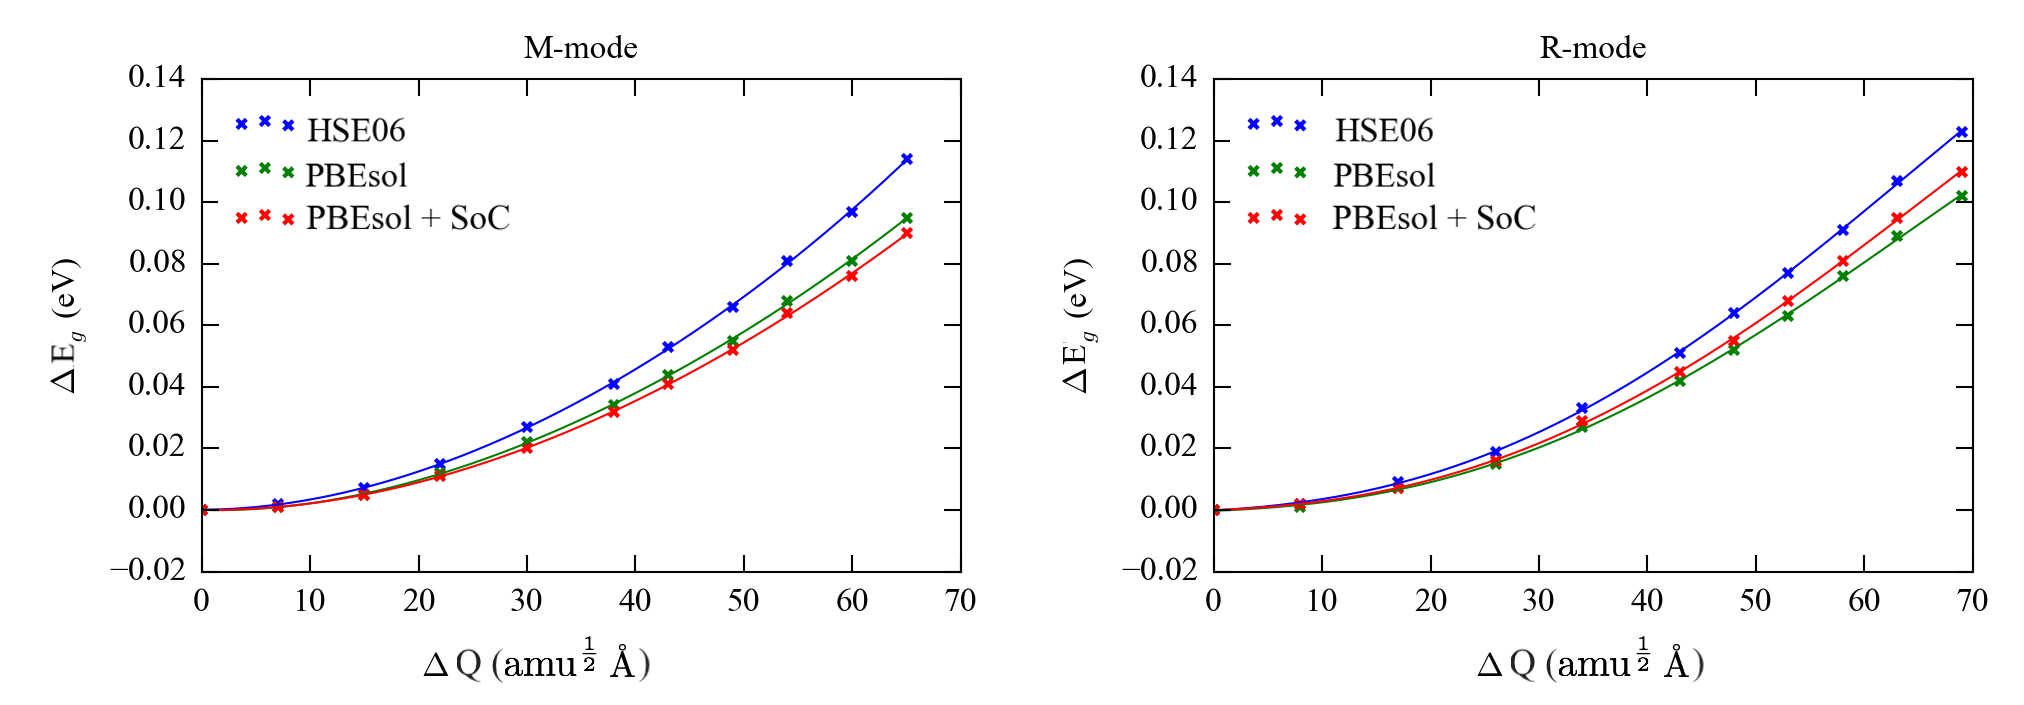
\includegraphics[width=\textwidth]{figures/ch5/fig_s4.png} 
\caption[Bandgap deformation potential at three levels of theory]{\label{Egtheory}
Change in bandgap ($\Delta E_\mathrm{g}$) as a function of the normal-mode coordinate $Q$ obtained with three exchange-correlation treatments used in the electronic-structure calculations, \textit{viz.} PBEsol, PBEsol with spin-orbit coupling (SoC), and HSE06.
}
\end{figure}

\begin{table*}\centering
\caption[Valence- and conduction-band deformation potentials]{
Valence- and conduction-band deformation potentials relative to the Pb 3d core energy level obtained from frozen-phonon calculations with three exchange-correlation treatments, \textit{viz.} PBEsol, PBEsol with spin-orbit coupling (SoC), and HSE06. We assume that the deformation potential is quadratic and fit a quadratic function $E=bQ^2$ to the band energies given in Figure\ \ref{ch5figs1}; the values in the table correspond to the coefficient $b$.
}
\begin{tabular}{ccccccccc} \label{ch5allxc} \\
\toprule
Mode & \hspace{5pt} & & \hspace{5pt} & PBEsol & \hspace{5pt} & PBEsol+SoC & \hspace{5pt} & HSE06 \\
\midrule
$M$ & & VBM & & $1.61 \times 10^{-5}$ & & $1.55 \times 10^{-5}$ & & $0.97 \times 10^{-5}$ \\
& & CBM & & $3.88 \times 10^{-5}$ & & $3.68 \times 10^{-5}$ & & $3.66 \times 10^{-5}$ \\ 
& & $\frac{CBM}{VBM}$ & & 2.14 &  & 2.37 & & 3.77  \vspace{5pt} \\

$R$ & & VBM & & $1.34 \times 10^{-5}$ & & $1.01 \times 10^{-5}$ & & $1.33 \times 10^{-5}$ \\
& & CBM & & $3.52 \times 10^{-5}$ & & $3.37 \times 10^{-5}$ & & $3.96 \times 10^{-5}$ \\
& & $\frac{CBM}{VBM}$ & & 2.63 & & 3.34 & & 2.98 \vspace{5pt} \\ 
\bottomrule
\end{tabular}
\end{table*}

% check how these deformation potentials have been calculated.

\subsubsection{Temperature dependant bandgap broadening} \label{ch5coupling}

The undistorted high-symmetry cubic perovskite structure is a saddle point between two equivalent broken-symmetry solutions (see Figure \ref{fig2}). Dynamic disorder is expected as the barriers are $37\ \textrm{meV}$ and $19\ \textrm{meV}$ for the $R$ and $M$ modes respectively, which is comparable to $k_\mathrm{B}T$. 
The Schr\"{o}dinger equation describing nuclear motion in the double well potential energy surface can be solved following a procedure outlined in Reference \cite{Skelton2016a}. 
The average bandgap as a function of temperature, $E_\mathrm{g}(T)$, can then be calculated from the thermally populated vibrational eigenstates $\chi(Q,T)$ that form a solution to the 1D Schr\"{o}dinger equation:
\begin{equation}
E_\mathrm{g}(T) = \langle \chi(Q,T)|E_\mathrm{g}(Q)|\chi(Q,T) \rangle
\end{equation}
Using this procedure, a positive band-gap shift of $35.5\ \textrm{meV}$ ($R$-mode) and $27.9\ \textrm{meV}$ ($M$-mode) at $T=300\ \textrm{K}$ has been calculated, which is comparable in magnitude to an experimentally measured broadening of $40\ \textrm{meV}$.\autocite{Wright2016} 
% And a note about the significance of this result?? Is it large??

\subsection{Hot carrier cooling to equilibium} \label{ch5:epcoupling}
In the previous subsection the coupling between the electronic and vibrational sub-systems was considered. This section focuses on the coupling between phonon modes, and how this relates to thermal transport in the material. The source of excess thermal energy is a hot polaronic state that is formed after above bandgap carrier excitation. The formation of a hot polaron is discussed first, followed by results for the cooling time to equilibrium.

\subsubsection{Hot polaron formation}
The Fr\"{o}lich polaron model has been recently recently applied to MAPI to calculate a polaron mobility from first principles.\autocite{Frost2017b} %Jarvist
When the polaron coupling is weak the kinetic energy is larger than the polaron binding energy, and the polaron radius is larger than a unit cell -- a large polaron is formed. When the polaron coupling is strong the electron is self-trapped, and the polaron radius is the size of a unit cell or smaller -- a small polaron is formed. The solution to the Fr\"{o}lich model in Reference \cite{Frost2017b} gives Fr\"{o}lich coupling constants of $\alpha=2.4$ and $\alpha=2.7$ for the electron and hole in MAPI, respectively. These values fall in the intermediate coupling regime where the large polaron model is valid, and correspond to a polaron radii of $26.8\AA$ for the electron and $25.3\AA$ for the hole, at \SI{300}{\K}.
Note that the calculated polaron radii are an upper bound, as bulk polaron states are further localised by disorder, point defects and extended defects such as surfaces, interfaces and grain boundaries.

In metals and other materials where the electron-phonon coupling is relatively homogeneous across the electron and phonon sub-systems, above-bandgap electrons cool over a single characteristic time scale.
The excited electrons lose their energy through phonon emission and the electron and phonon sub-systems are assumed to remain in distinct thermal equilibria, each described by time-dependent temperatures $T_{\mathrm{el}}(t)$ and $T_{\mathrm{ph}}(t)$. This is the two-temperature model.\autocite{Kaganov1955}
For materials where the electron-phonon coupling is heterogeneous, such as polar semiconductors with Fr\"{o}lich interactions, this model is not applicable, as the assumption that the phonon sub-system has reached a thermal equilibrium is not valid. 
For these materials, the above-bandgap electrons will transfer kinetic energy into the phonon modes which couple strongly to the electron sub-system, and these ``hot'' phonon modes will thermalise to a temperature above that of the remaining bulk modes. A recent computational study across 12 cubic semiconductors found that in each system studied there are hot phonon modes which equilibriate with the electron sub-system rather than with the phonon sub-system.\autocite{Sadasivam2017} This is in contrast to the two-temperature model where all phonons are in thermal equilibrium.

Transient spectroscopic studies\autocite{Klein2016,Price2015,Yang2016e} suggest that a hot photoexcited state persists in hybrid halide perovskites with a characteristic cooling time of up to \SI{100}{\pico\second}.
We consider the hot photoexcited state to be a Fr\"{o}lich polaron which resonates with a subpopulation of local phonon states; after polaron formation there is initial thermalisation, electron kinetic energy is transferred into the optical phonon modes and a hot polaron is formed.
This is a fast picosecond process via the strong Fr\"{o}lich coupling between the charge carrier and localised, polar phonon population. Once fully thermalised, the above bandgap energy is distributed amongst all phonon states associated with the polaron.

%include IPR as proof for cage modes?
The temperature of the resulting polaron depends on the polaron volume, the polaron specific heat capacity $C_v$ and the initial excitation energy (Figure \ref{ch5TemperatureRadius}). We assume that the polaron forms a sphere with a radius determined by the Fr\"{o}lich model (\SI{26.8}{\angstrom}) and that the initial excitation energy is distributed evenly between the electron and hole. 
The heat capacity is calculated from the bulk phonon calculation. Coupling to the optical cage modes ($\nu <$ \SI{5}{\tera\hertz}\autocite{Leguy2016}) at the gamma point are considered. The average temperature dependent energy $E(T)$ is determined by the phonon energies, $\epsilon_i = \hbar\nu_i$, and occupation numbers, as given by the Bose-Einstien distribution $n_i(T,\epsilon_i)$:
\begin{equation}
    E(T) = \sum_i \epsilon_i n_i(T,\epsilon_i) = \sum_i \frac{\epsilon_i}{\textrm{e}^{\frac{\epsilon_i}{k_\mathrm{B}T}}-1}.
\end{equation}
Following this, the specific heat capacity $C_v$ for a given temperature is given by:
\begin{equation}
    C_v = \frac{\partial E_T}{\partial T} = k_\mathrm{B} \sum_i \left(\frac{\epsilon_i}{k_\mathrm{B}T}\right)^2 \frac{\textrm{e}^{\frac{\epsilon_i}{k_\mathrm{B}T}}}{\left(\textrm{e}^{\frac{\epsilon_i}{k_\mathrm{B}T}}-1\right)^2}.
\end{equation}
%0.43454600, 0.75018732, 0.81515675, 0.89371517, 0.948438024, 1.01347671, 1.71280131, 1.97002626,1.99846539,2.20803605,2.34772924,2.73338668,3.52222265,3.82347645,3.99786503

For MAPI, the per-unit cell specific heat capacity is \SI{1.25}{\milli\eV\per\K} at
\SI{300}{\K}. Near-UV excitation at \SI{4}{\eV} gives a maximum energy of \SI{1.2}{\eV} which can be transferred to the polaron, and the temperature increases with localisation ($T \propto r^{-3}$).

\begin{figure}[h]
\centering
  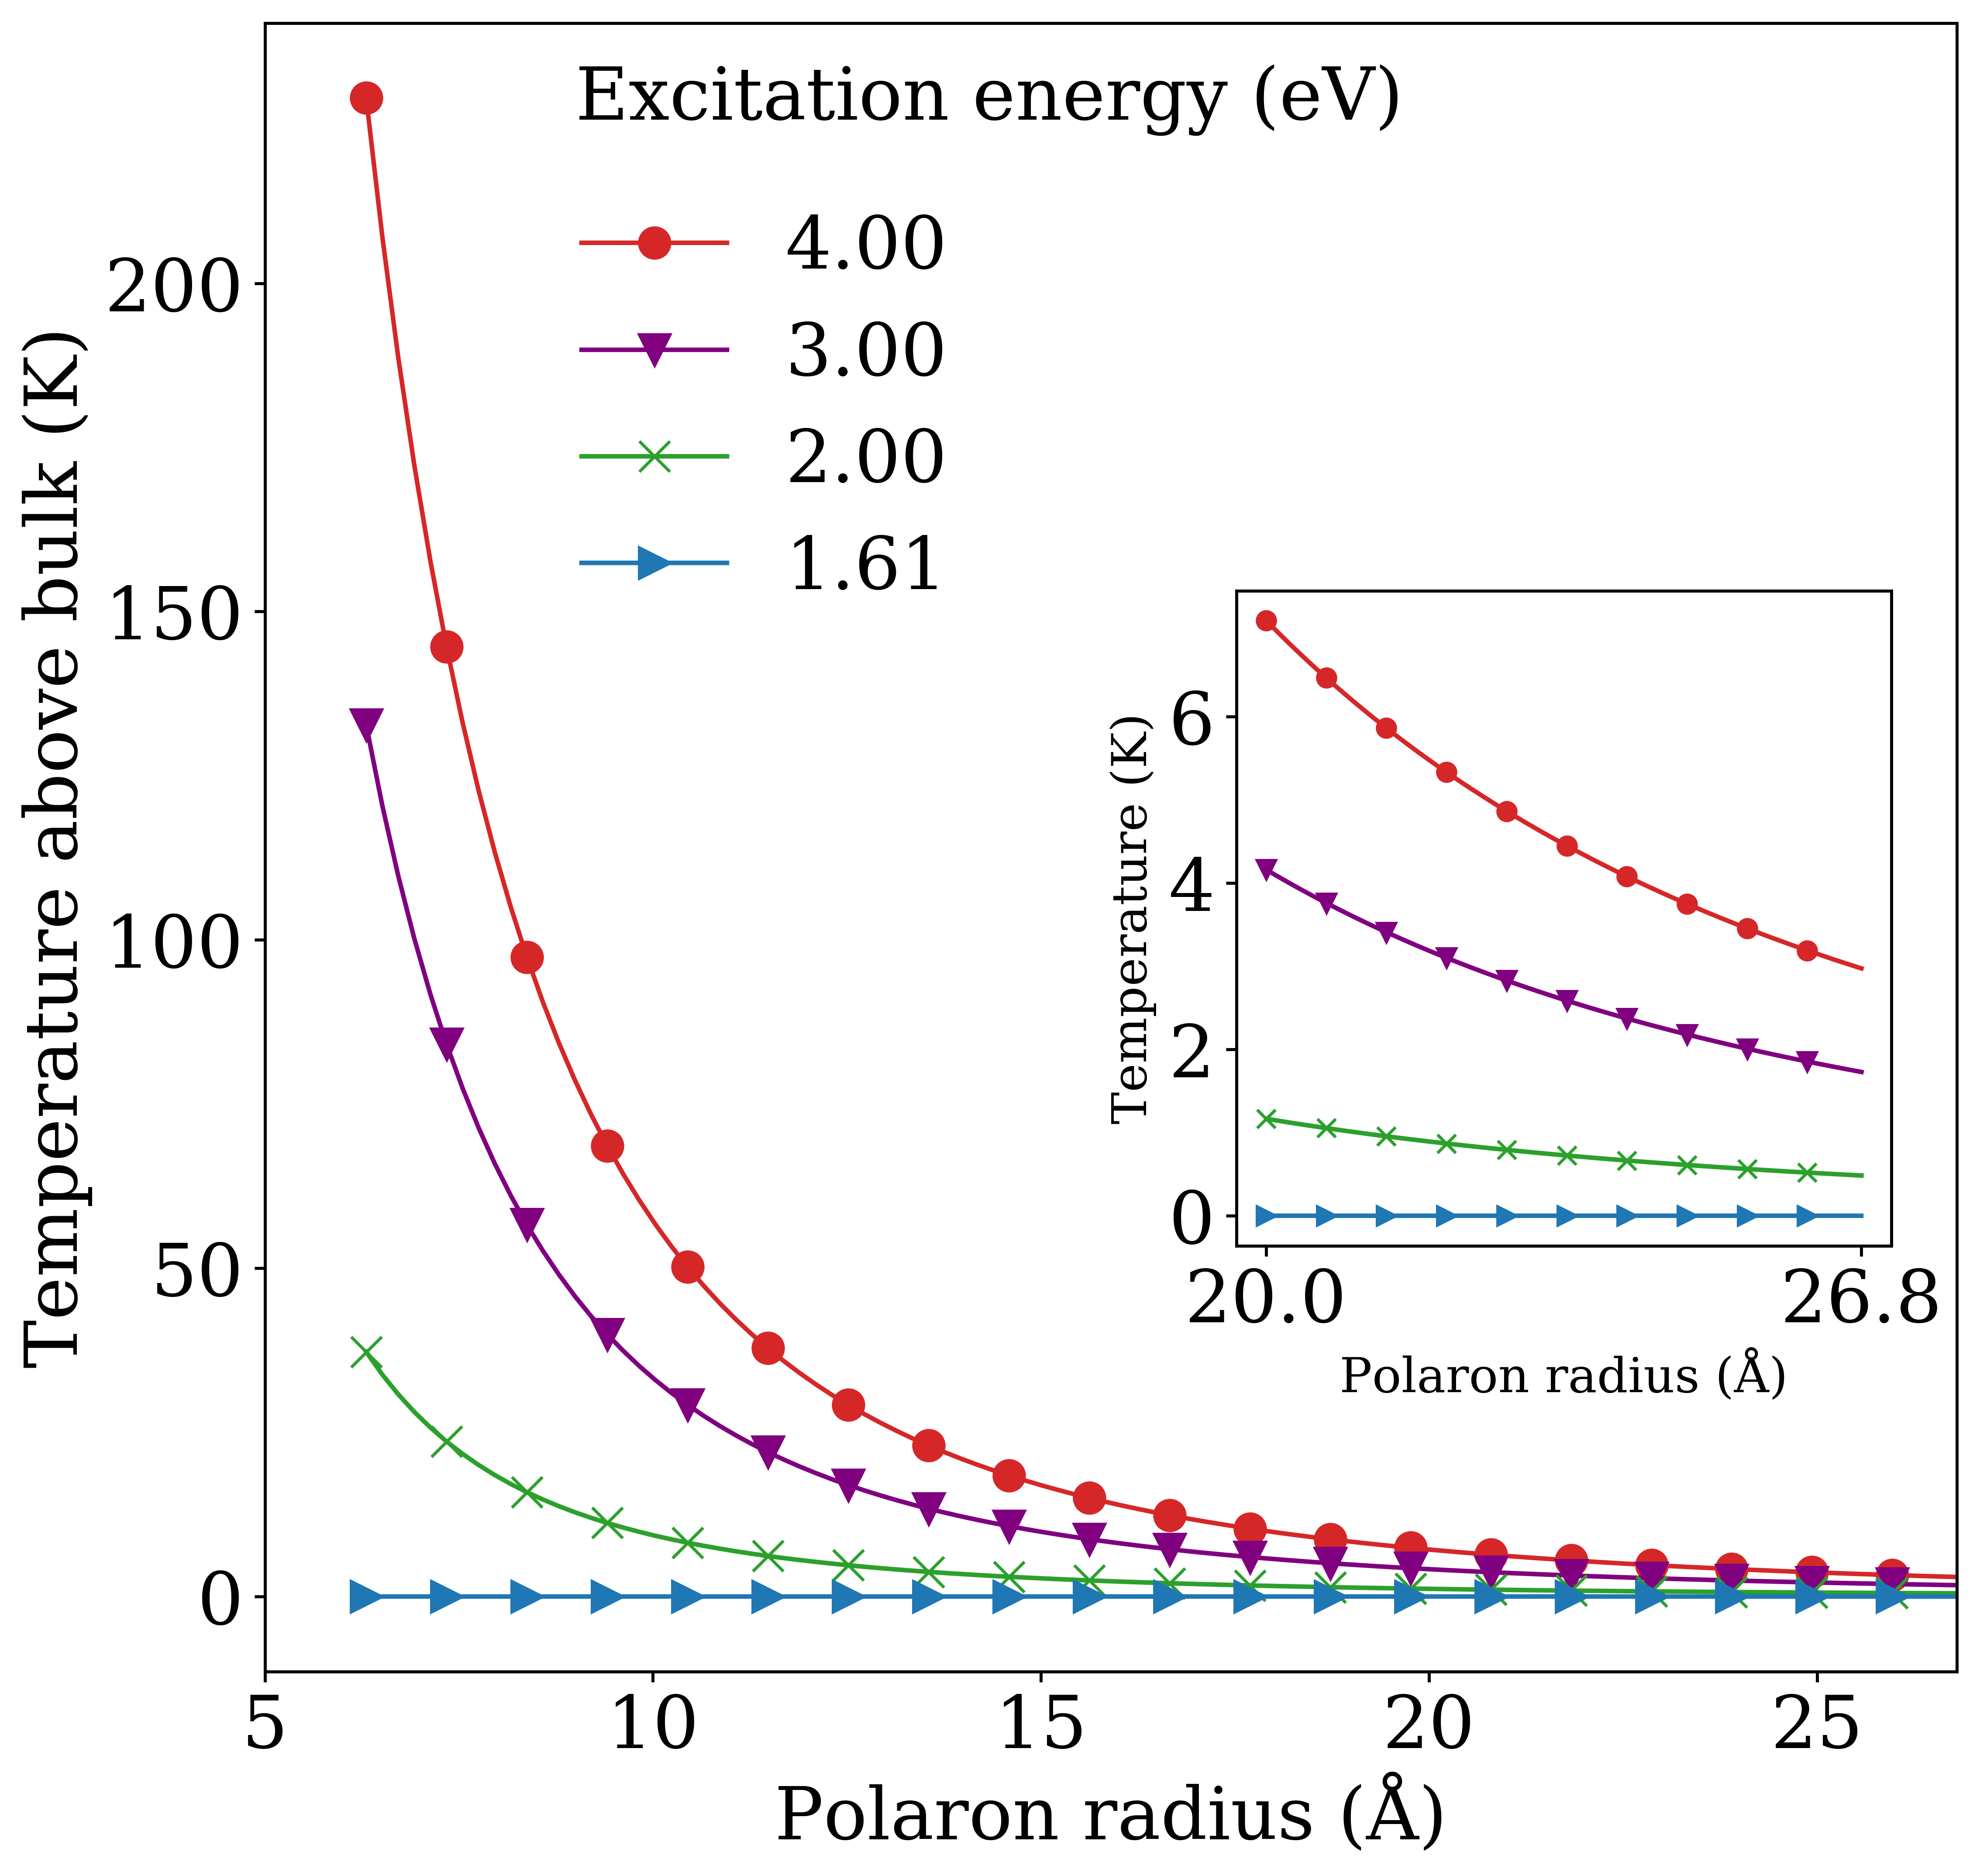
\includegraphics[width=0.7\textwidth]{figures/ch5/f3.png}
  \caption[Polaron temperature as a function of polaron radius]{Thermalised polaron temperature in MAPI as a function of polaron radius and excitation energy assuming a bulk value of the heat capacity. The calculated bulk electron polaron radius of \SI{26.8}{\angstrom} provides an upper bound for polaron size. The lattice parameter (\SI{6.3}{\angstrom}) is used as a lower bound -- below this the continuum large polaron approach is not valid. Excitation from the bandgap to near-UV are considered. Inset shows detail at larger radii (axes same as main). }
  \label{ch5TemperatureRadius}
\end{figure}

% how we calculate teh specific heat. The theory has been outlined clearly by Jarvist Frost, and Independantly verified by myself.

\subsubsection{Cooling to equilibrium}
After a fast initial thermalisation, the polaron will cool to equilibrium over a longer timeframe. During this cooling process the excited local optical phonon modes scatter into phonon modes that diffuse away from the polaron.

Due to energy and momentum conservation rules, three-phonon scattering is the lowest-order scattering process.  The three-phonon interaction strengths have been calculated for MAPI,\autocite{Whalley2016} and they are found to be orders of magnitude stronger than for CdTe and GaAs. In addition, there are a large number of energy- and momentum conserving scattering pathways. As a result the bulk thermal conductivity, calculated from a solution of the Boltzmann transport equation in the relaxation time approximation, is extremely low; \SI{0.05}{\watt\per\metre\per\K} at \SI{300}{\K}.\autocite{Whalley2016} 
In contrast, the calculated conductivity for GaAs and CdTe is 
\SI{38}{\watt\per\metre\per\K}
and
\SI{9}{\watt\per\metre\per\K},
respectively.

\begin{figure}[h]
\centering
  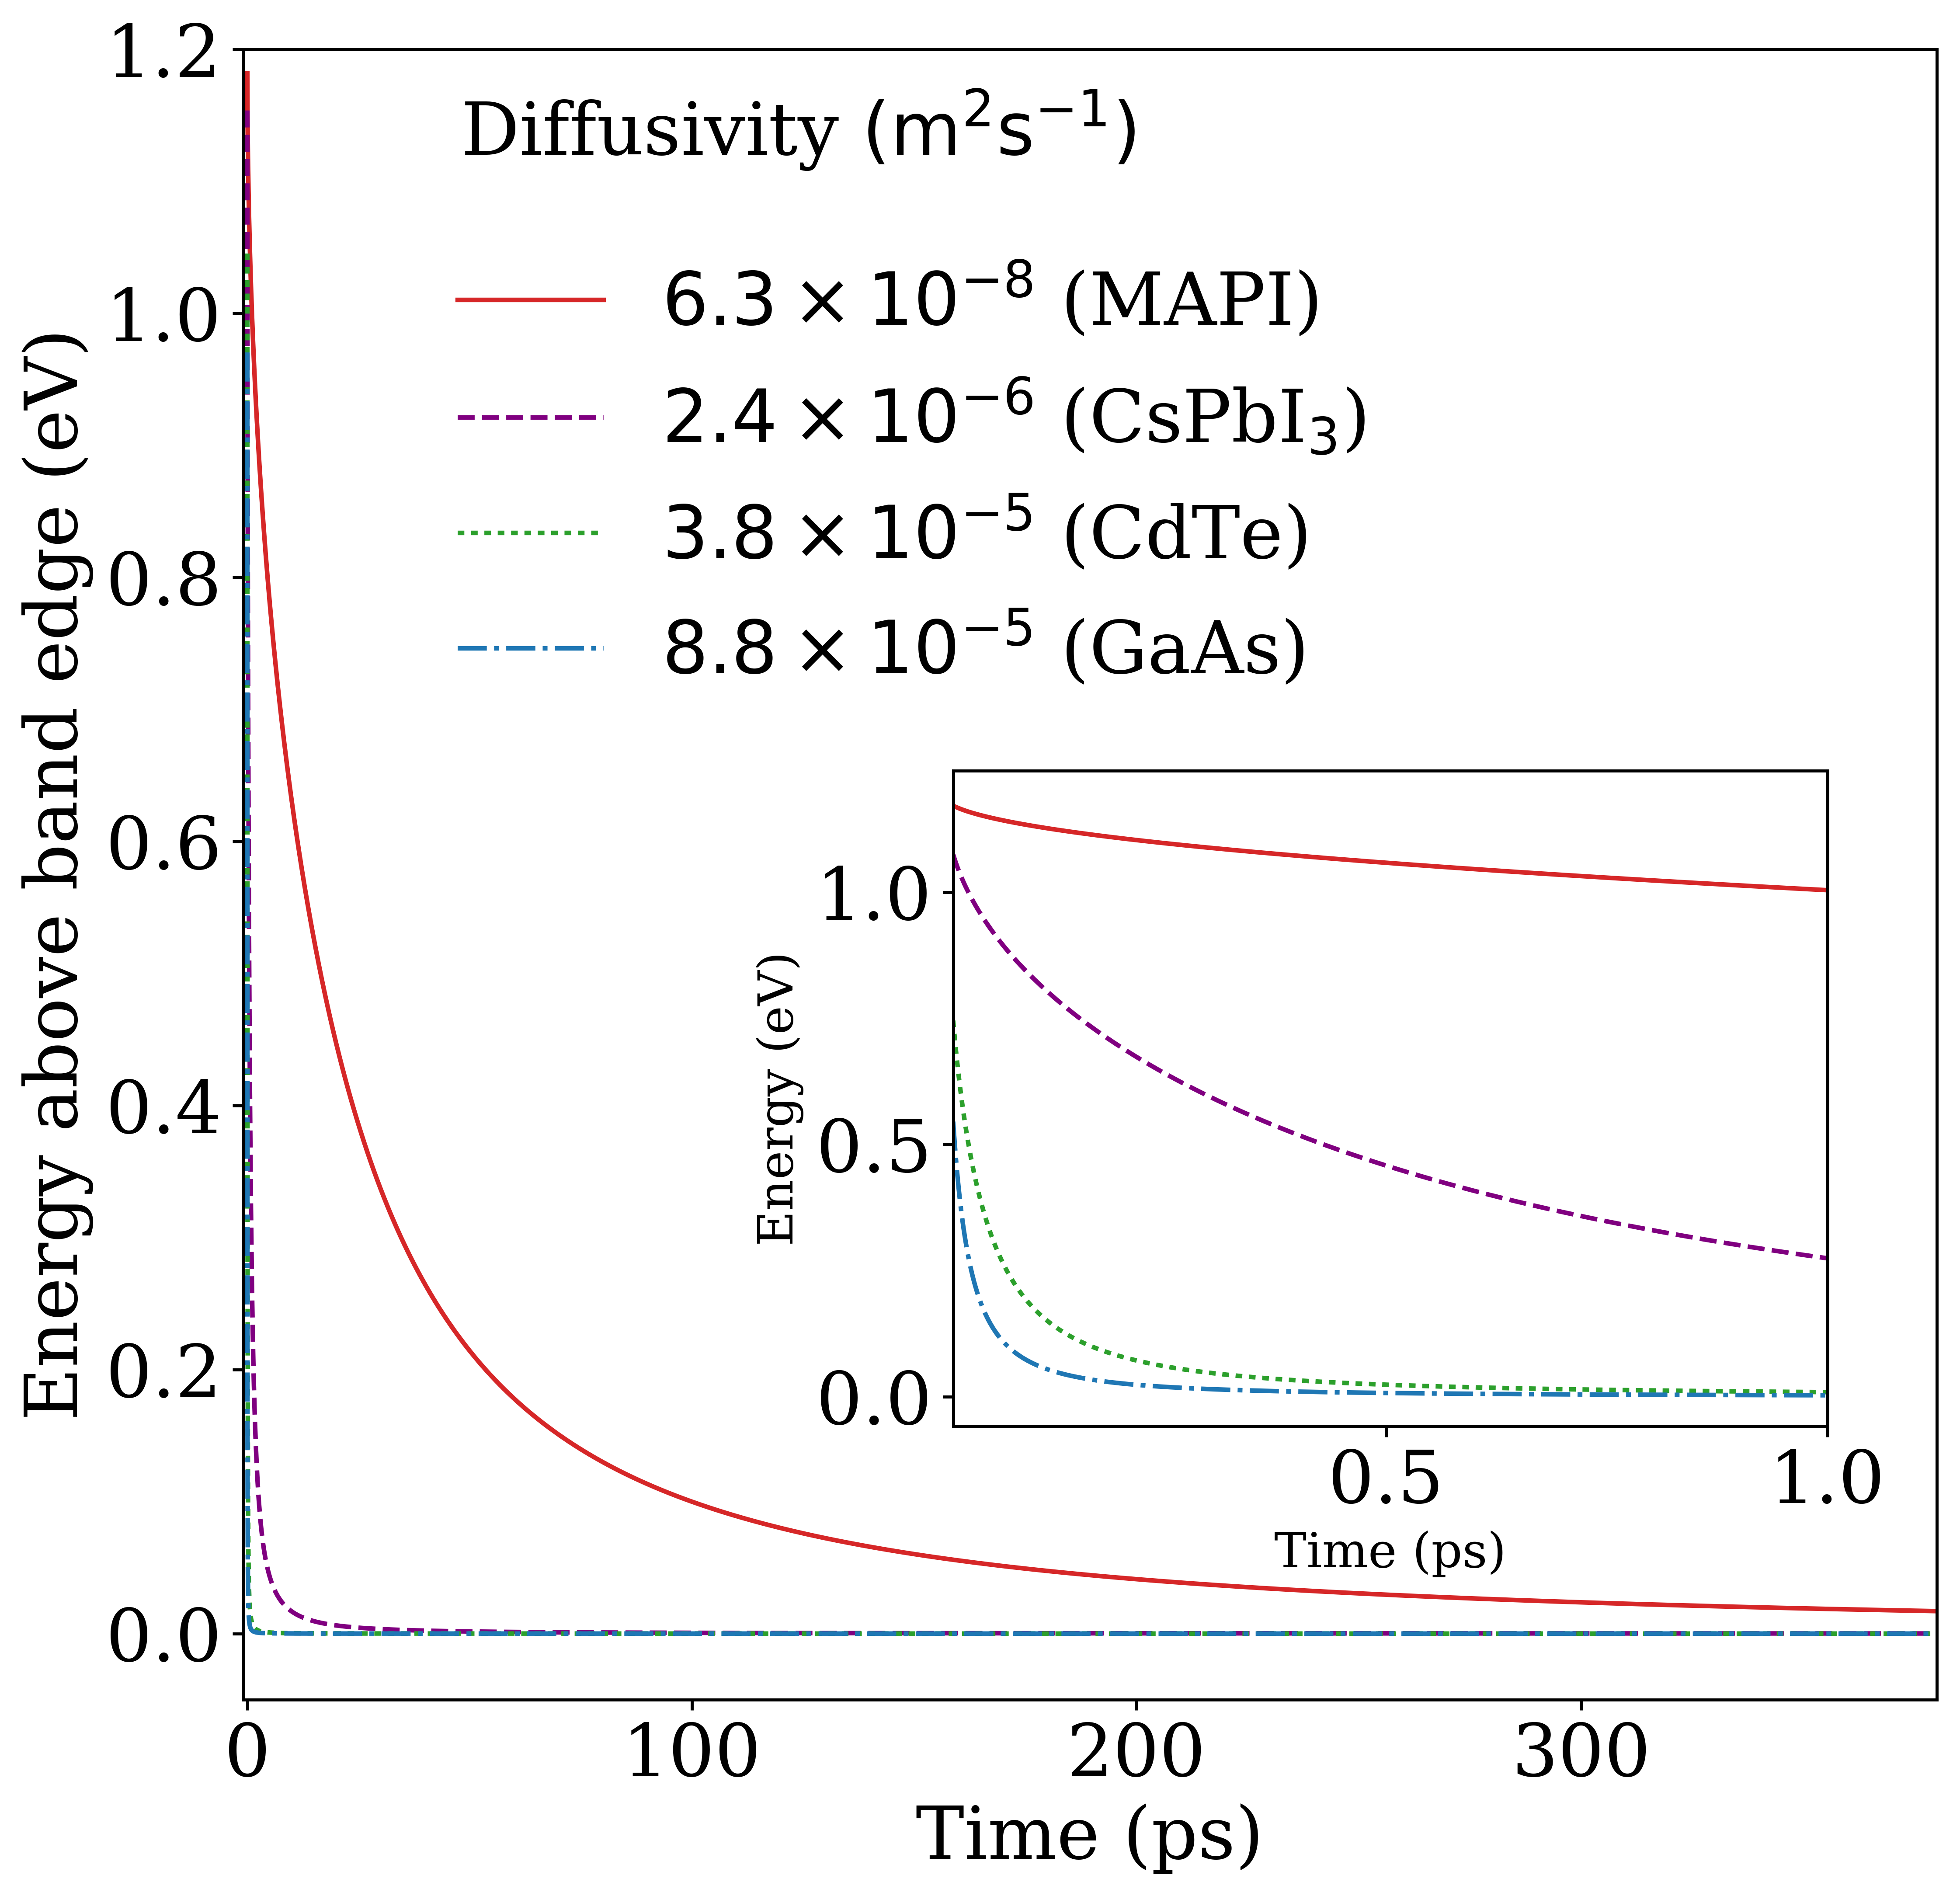
\includegraphics[width=0.6\textwidth]{figures/ch5/f4.png}
  \caption[Hot carrier cooling rate]{The energy of a large polaron state (starting at \SI{1.2}{\electronvolt} above the conduction band minimum, with a polaron radius of \SI{26.8}{\angstrom}) in \ce{CH3NH3PbI3} as a function of time. The slow rate is due to the low thermal conductivity in MAPI ($\kappa=$\SI{0.05}{\watt\per\metre\per\K}). For comparison, we show the behaviour using the thermal conductivities of CdTe ($\kappa$ = 9) and GaAs ($\kappa$ = 38). }
  \label{ch5TemperatureTime}
\end{figure}

To model the third order phonon-phonon scattering processes we consider the polaron as a hot sphere in a continuum of ambient temperature material, which allows us to calculate temperature as a function of time using the heat diffusion equation.
We consider the low fluence limit where individual photon quanta are absorbed into isolated hot polarons.
The rate of cooling is determined by the diffusivity $D$: 
\begin{equation}
    D= \frac{\kappa}{\rho C_p},
\end{equation} 
where $\kappa$ is the thermal conductivity, $\rho$ is the density and $C_p$ is the specific heat capacity. 

Heat diffuses from MAPI on the order of  \SI{100}{\pico\second}, whilst for other conductivities the process is much faster, on the order of \SI{100}{\femto\second}. 
This is in agreement with reported experimental values from References \cite{Klein2016} (MAPI), \cite{Zhong2017} (CdTe) and \cite{Rosenwaks1993} (GaAs). 
Note that at short timescales, measurements of hot carrier cooling in MAPI and \ce{CsPbI3} ($\kappa$ = 0.5) may appear linear due to the slower exponential decay.

\section{Summary}

In this chapter we have introduced the phonon quasi-particle into our description of MAPI. The first consequence of this is that the electronic states couple to the normal mode vibrations of the system. I have quantified the extent of this coupling to two highly anharmonic phonon modes at the $M$ and $R$ points in the Brillouin Zone. These modes, which are occupied at room temperature, have a large amplitude of motion and lead to a bandgap broadening comparable to that found experimentally -- i.e. they play a significant role in the overall electron-phonon coupling of the system.
The second consequence of including phonons in our model is that temperature variations in the bulk material lead to heat diffusion. I have shown that a classical heat diffusion model, parameterised using Fr\"{o}lich polaron theory and first-principles calculations, can be used to
describe the physical process behind the experimentally observed slow hot-carrier cooling rates
observed for halide perovskites.

\textbf{Data Access Statement}

The crystal structures and phonon data are available at \url{https://github.com/WMD-group/Phonons}, 
and can be processed using the \textsc{phonopy}\autocite{Togo2015} and  \textsc{modemap}\autocite{ModeMap} packages. For visualising the phonon modes the \textsc{ascii phonons} package can be used.\autocite{asciiphonons} The phonon dispersion can be plotted using the \textsc{sumo} package.\autocite{sumo2018}

Data files and Jupyter notebooks outlining the calculation steps for hot carrier cooling are available as a repository on GitHub at \url{https://github.com/WMD-group/hot-carrier-cooling}.

\textbf{Acknowledgements}

Via our membership of the UK's HEC Materials Chemistry Consortium, which is funded by EPSRC (EP/L000202), this work used the ARCHER UK National Supercomputing Service (http://www.archer.ac.uk). I also made use of the Balena HPC facility at the University of Bath, which is maintained by Bath University Computing Services. 


